\section{Experimental Results}  \label{sec:exp}

\subsection{Experimental Setup}

\subsubsection{Datasets}

\paragraph*{Berkeley Dataset}

The Intel Berkeley Research lab dataset~\cite{berkeley2004lab} records temperature, humidity, light, and voltage for 54 sensors (with 1 missing completely missing) for which locations are given (see Figure \ref{berkeley_lab}).
The dataset includes 2.3M sensor observations, over 210K timesteps, and was recorded between February 28th and April 5th, 2004 in an indoor lab environment.

\begin{figure}[H]
\centering
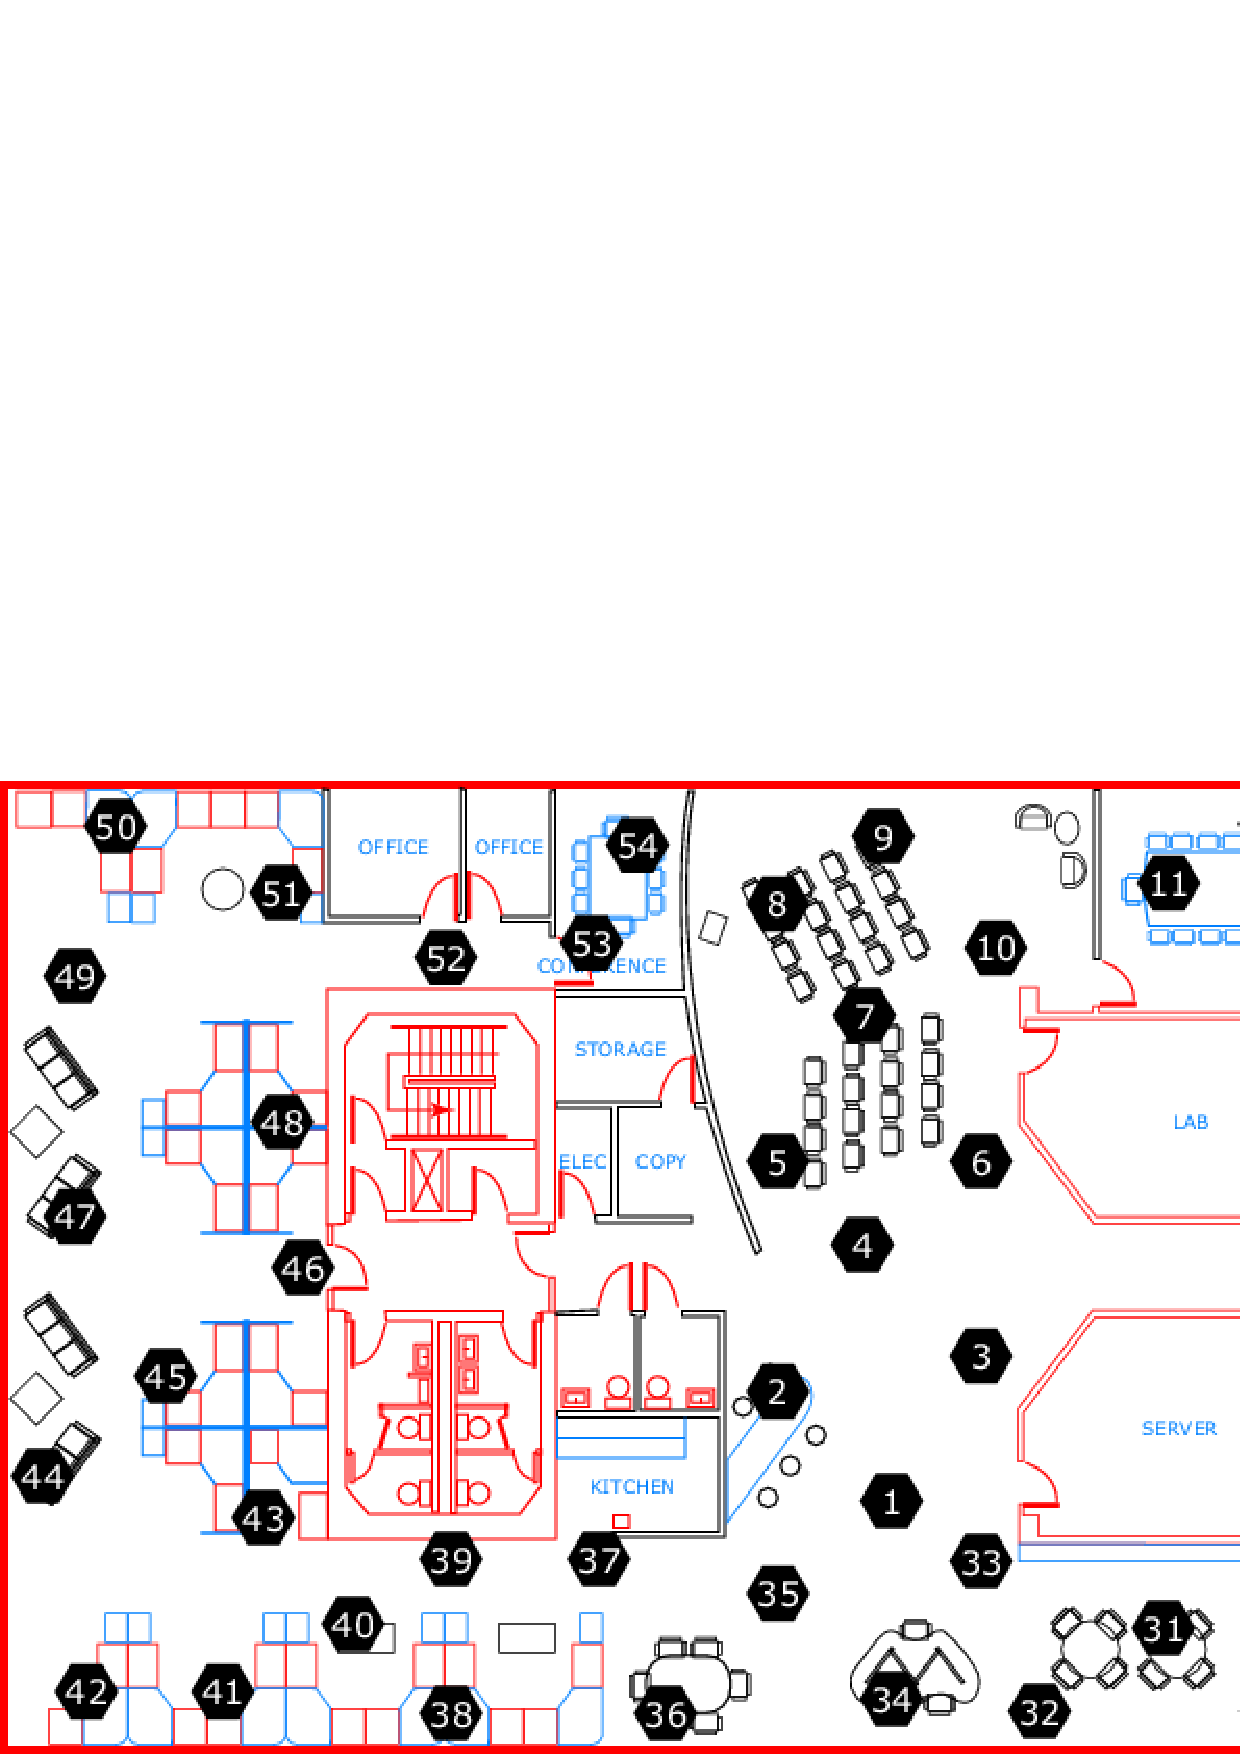
\includegraphics[scale=0.25]{berkeley_lab.png}
\caption{Intel Berkeley Research Lab Floorplan} \label{berkeley_lab}
\end{figure}

\paragraph*{Traffic Dataset}

The Traffic Dataset records the temperature, humidity, and voltage conditions of 20 sensor nodes and one gateway node.
This dataset, collected by the Bio-industrial Department at National Taiwan University, was recorded over a 2.5 year time period ending in 2011 in an outdoor location high traffic area in Taipei, Taiwan. \redtext{Include citation for Traffic Dataset! (Chun contacting authors)}

\begin{figure}[H]
\centering
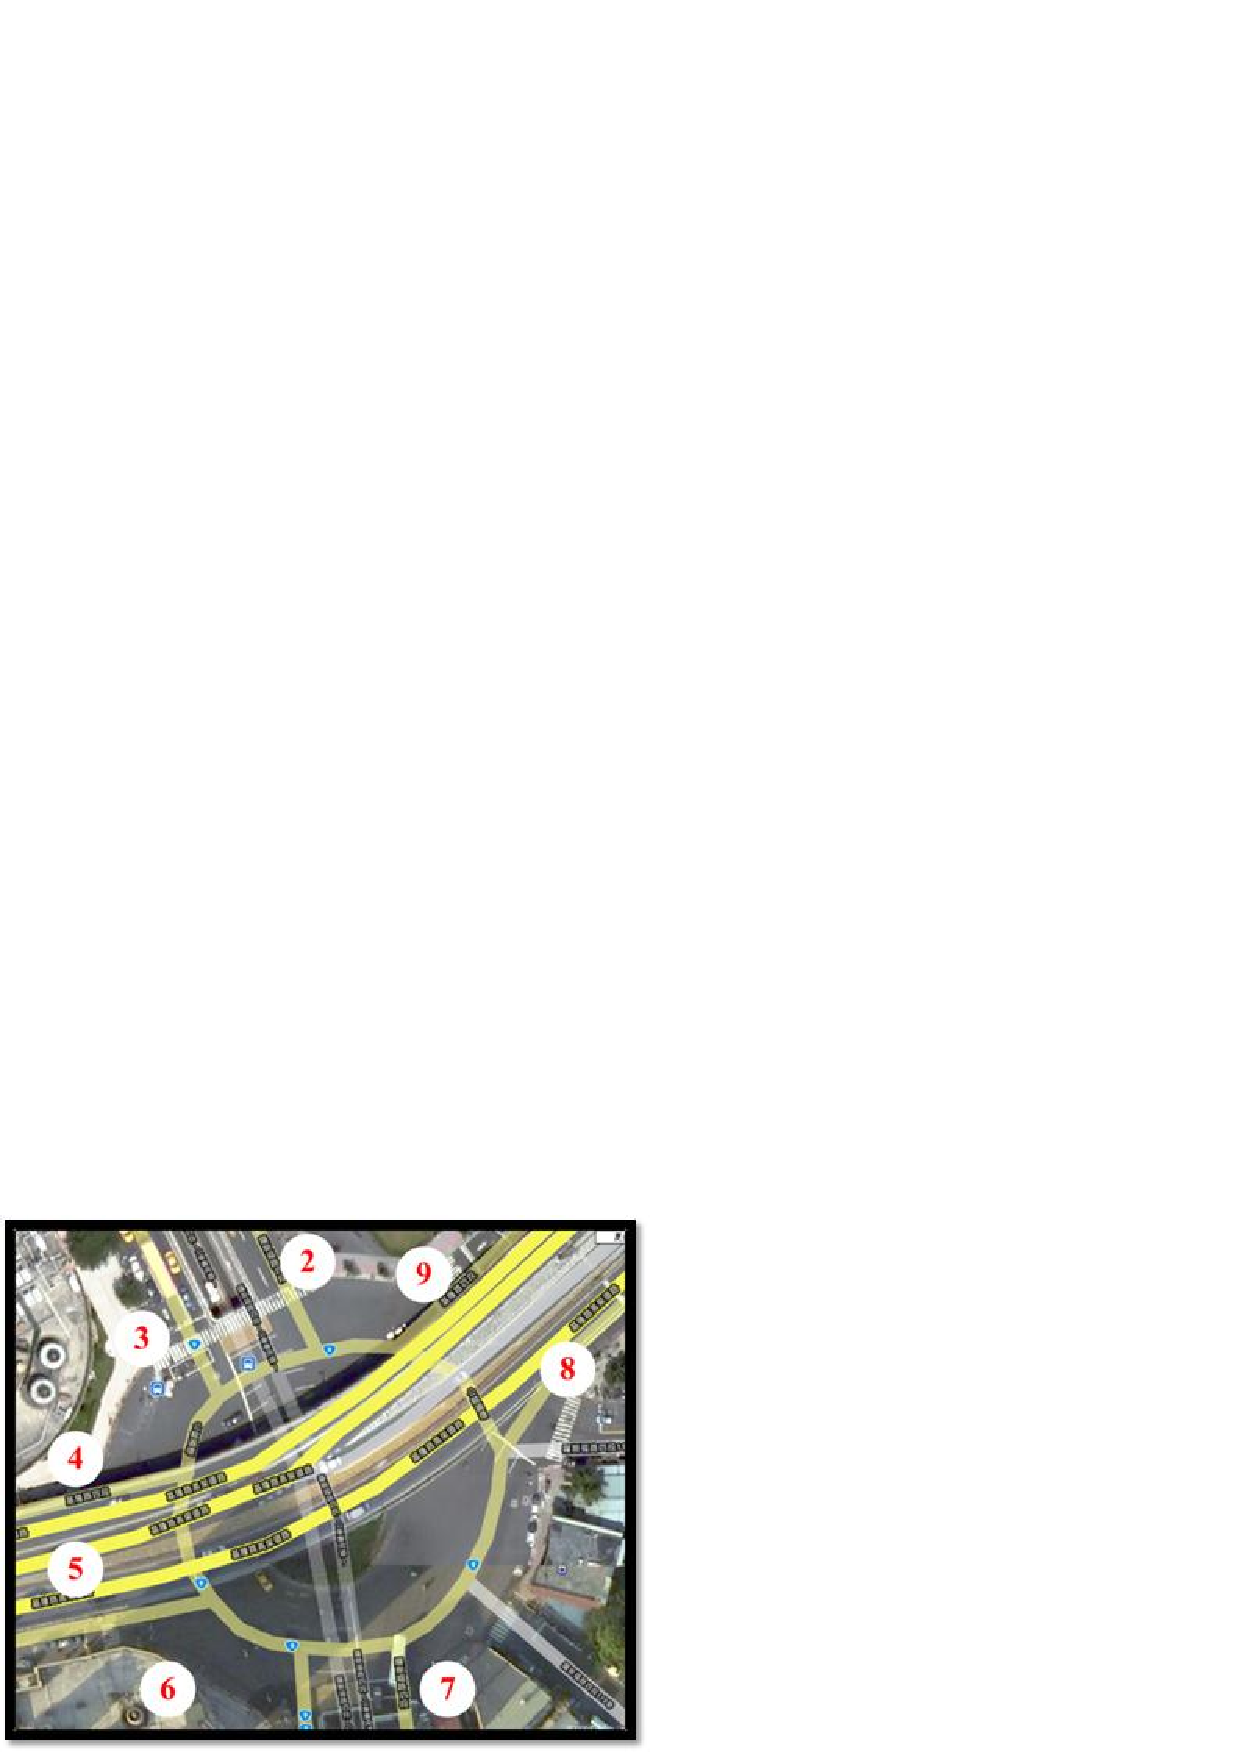
\includegraphics[scale=0.5]{traffic_wsn.png}
\caption{Traffic Sensor Deployment Configuration (7 sensors of 20 shown)}
\end{figure}

\subsubsection{Dataset Preparation}

\paragraph*{Berkeley Dataset Outlier Removal and Gridding}

Outlier Filtering : Observation removed if temperature $> 100\degc$, temperature $< 5\degc$, or humidity $< 16\%$.

Gridding : Dataset falls on even 30s intervals for the first 5000 time steps (which is all we consider), so no additional gridding need be performed.

\paragraph*{Traffic Dataset Outlier Removal and Gridding}

Outlier Filtering : \redtext{this was done by chung-yi.. please fill this in!}

Gridding : The original dataset recorded most readings at around the $xx:03$ and $xx:33$ minute marks, so a $6$ min window centered at
these points captured the data for $30$ minute internal readings.
Where more than one reading was recorded for a given node within a given window, the closest to the $3$ or $33$ minute mark was chosen.
The full length of the dataset was used, which consists of $~43$K time-steps.

\paragraph*{Common Methodology}

%Datasets of various lengths are produced from the single input dataset for our experiments, namely 2500, 5000, and 10000.
There is an initially missing portion of the observations which can be considered Missing At Random (MAR).
To this, we impose two different types of Missing Completely At Random (MCAR) sampling techniques to build validation and testing datasets.

\paragraph*{Random Missing Pattern}

This pattern reflects choosing a random time and random sensor to be missing and hence removed from the training set.
We define two values $x$ and $y$ as follows.

\begin{itemize}
\item $10\%$ of the non-missing data is randomly selected (without replacement) to be the validation set
\item $y\%$ of the non-missing data is randomly selected (without replacement) to be the testing set
\item The remaining data is part of the training set (this would be $x\%$ of the total data given no missing; assuming missing rate of $m\%$, the actual data in training set is $90\%-x\%-m\%$
\end{itemize}

\paragraph*{Temporal Missing Pattern}

This pattern reflects testing the effect of all data missing after a certain point in time.
We define two values $x$ and $y$ as follows.

\begin{itemize}
\item Here, we have the last $y\%$ of time is in test and the prior $10\%$ to test is the validation.
\item The sensor node numbers ``covered up'' in the validation and testing for the Berkeley and Traffic datasets are ${2,4,6,8,10,14,17,19,20,99}$ and ${4,21,45}$, respectively.
\end{itemize}

\subsection{Basic Experimental Results} %from Chung-Yi
We compare linear interpolation~(LI), TRMF, AKE, DESM and STI on the two data sets. Note that the sensor location information is not available in traffic data set, so we assume the distance between all sensor node pairs are equal for DESM and STI.

%validation setting
\subsubsection{Random Split}
Table \ref{table:berkeley_random_hum}, \ref{table:berkeley_random_light} and \ref{table:berkeley_random_tem} show the result of random split on Berkeley data set. TRMF outperforms others greatly in all cases. On the other hand, linear interpolation is quite competitive, especially when the size of training set is large. This is because the sampling rate of Berkeley data set is fairly high and the temporal correlation is prominent. 

\begin{table}[htbp]
\centering
\caption{RMSE of (Berkeley, random, humidity)}
\label{table:berkeley_random_hum}
\begin{tabular}{ r | r r r r r}
	train	&LI	&TRMF	&AKE	&DESM	&STI\\ \hline
	10\% & $ 0.171_{(2)} $ & $ \mathbf{ 0.142_{(1)} } $ & $ 0.264_{(3)} $ & $ 0.544_{(4)} $ & $ 1.220_{(5)} $ \\
	20\% & $ 0.127_{(2)} $ & $ \mathbf{ 0.114_{(1)} } $ & $ 0.244_{(3)} $ & $ 0.318_{(4)} $ & $ 1.472_{(5)} $ \\
	40\% & $ 0.095_{(2)} $ & $ \mathbf{ 0.092_{(1)} } $ & $ 0.199_{(3)} $ & $ 0.219_{(4)} $ & $ 1.648_{(5)} $ \\
	60\% & $ 0.085_{(2)} $ & $ \mathbf{ 0.082_{(1)} } $ & $ 0.181_{(4)} $ & $ 0.180_{(3)} $ & $ 1.649_{(5)} $ \\
	80\% & $ \mathbf{ 0.075_{(1)} } $ & $ 0.076_{(2)} $ & $ 0.127_{(3)} $ & $ 0.160_{(4)} $ & $ 1.604_{(5)} $ \\
	85\% & $ \mathbf{ 0.074_{(1)} } $ & $ 0.075_{(2)} $ & $ 0.121_{(3)} $ & $ 0.148_{(4)} $ & $ 1.549_{(5)} $ \\ \hline
	rank &1.67 &1.33 &3.17 &3.83 &5.00 \\
\end{tabular}
\end{table}

\begin{table} [htbp]
\centering
\caption{RMSE of (Berkeley, random, light)}
\label{table:berkeley_random_light}
\begin{tabular}{ r |  r r r r r}
	train	&LI	&TRMF	&AKE	&DESM	&STI\\ \hline
	10\% & $ 52.9_{(2)} $ & $ \mathbf{ 35.5_{(1)} } $ & $ 61.2_{(3)} $ & $ 6250.4_{(5)} $ & $ 258.2_{(4)} $ \\
	20\% & $ 38.7_{(2)} $ & $ \mathbf{ 28.2_{(1)} } $ & $ 53.0_{(3)} $ & $ 215.9_{(4)} $ & $ 311.0_{(5)} $ \\
	40\% & $ 29.9_{(2)} $ & $ \mathbf{ 21.2_{(1)} } $ & $ 41.4_{(3)} $ & $ 356.7_{(5)} $ & $ 356.3_{(4)} $ \\
	60\% & $ 25.0_{(2)} $ & $ \mathbf{ 17.2_{(1)} } $ & $ 33.7_{(3)} $ & $ 112.6_{(4)} $ & $ 366.9_{(5)} $ \\
	80\% & $ 23.9_{(2)} $ & $ \mathbf{ 17.7_{(1)} } $ & $ 27.9_{(3)} $ & $ 41.7_{(4)} $ & $ 363.3_{(5)} $ \\
	85\% & $ 20.9_{(2)} $ & $ \mathbf{ 14.4_{(1)} } $ & $ 24.3_{(3)} $ & $ 44.4_{(4)} $ & $ 354.2_{(5)} $ \\ \hline
	rank &2.00 &1.00 &3.00 &4.33 &4.67 \\
\end{tabular}
\end{table}

\begin{table}[htbp]
\centering
\caption{RMSE of (Berkeley, random, temperature)}
\label{table:berkeley_random_tem}
\begin{tabular}{ r | r r r r r}
	train	&LI	&TRMF	&AKE	&DESM	&STI\\ \hline
	10\% & $ 0.070_{(2)} $ & $ \mathbf{ 0.046_{(1)} } $ & $ 0.112_{(3)} $ & $ 0.298_{(4)} $ & $ 0.506_{(5)} $ \\
	20\% & $ 0.042_{(2)} $ & $ \mathbf{ 0.032_{(1)} } $ & $ 0.111_{(3)} $ & $ 0.167_{(4)} $ & $ 0.584_{(5)} $ \\
	40\% & $ 0.027_{(2)} $ & $ \mathbf{ 0.023_{(1)} } $ & $ 0.080_{(3)} $ & $ 0.095_{(4)} $ & $ 0.644_{(5)} $ \\
	60\% & $ 0.021_{(2)} $ & $ \mathbf{ 0.018_{(1)} } $ & $ 0.053_{(3)} $ & $ 0.067_{(4)} $ & $ 0.637_{(5)} $ \\
	80\% & $ 0.016_{(2)} $ & $ \mathbf{ 0.015_{(1)} } $ & $ 0.043_{(3)} $ & $ 0.048_{(4)} $ & $ 0.611_{(5)} $ \\
	85\% & $ 0.019_{(2)} $ & $ \mathbf{ 0.016_{(1)} } $ & $ 0.034_{(3)} $ & $ 0.048_{(4)} $ & $ 0.593_{(5)} $ \\ \hline
	rank &2.00 &1.00 &3.00 &4.00 &5.00 \\
\end{tabular}
\end{table}

Table \ref{table:traffic_random_hum} and \ref{table:traffic_random_tem} show the result of random split on traffic data set. Again, TRMF outperforms other models significantly. However, the performance of linear interpolation deteriorates a lot. This corresponds to the low sampling rate in traffic data set. 

\begin{table} [htbp]
\centering
\caption{RMSE of (traffic, random, humidity)}
\label{table:traffic_random_hum}
\begin{tabular}{ r | r r r r r}
	train	&LI	&TRMF	&AKE	&DESM	&STI\\ \hline
	10\% & $ 11.630_{(4)} $ & $ \mathbf{ 3.524_{(1)} } $ & $ 7.307_{(2)} $ & $ 19.817_{(5)} $ & $ 10.625_{(3)} $ \\
	20\% & $ 7.269_{(4)} $ & $ \mathbf{ 2.583_{(1)} } $ & $ 4.559_{(2)} $ & $ 14.634_{(5)} $ & $ 6.745_{(3)} $ \\
	40\% & $ 4.233_{(3)} $ & $ \mathbf{ 1.932_{(1)} } $ & $ 3.458_{(2)} $ & $ 8.986_{(5)} $ & $ 5.021_{(4)} $ \\
	60\% & $ 3.184_{(3)} $ & $ \mathbf{ 1.664_{(1)} } $ & $ 2.901_{(2)} $ & $ 6.396_{(5)} $ & $ 4.710_{(4)} $ \\
	80\% & $ 2.690_{(3)} $ & $ \mathbf{ 1.565_{(1)} } $ & $ 2.511_{(2)} $ & $ 4.714_{(5)} $ & $ 4.605_{(4)} $ \\
	85\% & $ 2.588_{(3)} $ & $ \mathbf{ 1.503_{(1)} } $ & $ 2.401_{(2)} $ & $ 4.382_{(4)} $ & $ 4.671_{(5)} $ \\ \hline
	rank &3.33 &1.00 &2.00 &4.83 &3.83 \\
\end{tabular}
\end{table}

\begin{table} [htbp]
\centering
\caption{RMSE of (traffic, random, temperature)}
\label{table:traffic_random_tem}
\begin{tabular}{ r | r r r r r}
	train	&LI	&TRMF	&AKE	&DESM	&STI\\ \hline
	10\% & $ 4.000_{(4)} $ & $ \mathbf{ 1.214_{(1)} } $ & $ 2.509_{(2)} $ & $ 6.212_{(5)} $ & $ 3.662_{(3)} $ \\
	20\% & $ 2.508_{(4)} $ & $ \mathbf{ 0.898_{(1)} } $ & $ 1.538_{(2)} $ & $ 4.867_{(5)} $ & $ 2.261_{(3)} $ \\
	40\% & $ 1.477_{(3)} $ & $ \mathbf{ 0.689_{(1)} } $ & $ 1.192_{(2)} $ & $ 3.149_{(5)} $ & $ 1.732_{(4)} $ \\
	60\% & $ 1.101_{(3)} $ & $ \mathbf{ 0.585_{(1)} } $ & $ 1.005_{(2)} $ & $ 2.275_{(5)} $ & $ 1.597_{(4)} $ \\
	80\% & $ 0.938_{(3)} $ & $ \mathbf{ 0.551_{(1)} } $ & $ 0.885_{(2)} $ & $ 1.702_{(5)} $ & $ 1.574_{(4)} $ \\
	85\% & $ 0.915_{(3)} $ & $ \mathbf{ 0.519_{(1)} } $ & $ 0.866_{(2)} $ & $ 1.494_{(4)} $ & $ 1.585_{(5)} $ \\ \hline
	rank &3.33 &1.00 &2.00 &4.83 &3.83 \\
\end{tabular}
\end{table}

\subsubsection{Temporal Split}
Table \ref{table:berkeley_temporal_hum}, \ref{table:berkeley_temporal_light} and \ref{table:berkeley_temporal_tem} show the result of temporal split on Berkeley data set and Table \ref{table:traffic_temporal_hum} and \ref{table:traffic_temporal_tem} show the result of temporal split on traffic data set.
In the temporal split, it is clear that linear interpolation performs terribly since its prediction is simply the last reading of the sensor.

\begin{table}[htbp]
\centering
\caption{RMSE of (Berkeley, temporal, humidity)}
\label{table:berkeley_temporal_hum}
\begin{tabular}{ r | r r r r r}
	train	&LI	&TRMF	&AKE	&DESM	&STI\\ \hline
	10\% & $ 4.183_{(4)} $ & $ 0.957_{(2)} $ & $ 1.669_{(3)} $ & $ 4.185_{(5)} $ & $ \mathbf{ 0.792_{(1)} } $ \\
	20\% & $ 5.421_{(4)} $ & $ \mathbf{ 0.796_{(1)} } $ & $ 0.969_{(3)} $ & $ 5.422_{(5)} $ & $ 0.865_{(2)} $ \\
	40\% & $ 6.443_{(4)} $ & $ \mathbf{ 0.771_{(1)} } $ & $ 1.025_{(3)} $ & $ 6.443_{(5)} $ & $ 0.961_{(2)} $ \\
	60\% & $ 2.223_{(4)} $ & $ \mathbf{ 0.540_{(1)} } $ & $ 0.928_{(3)} $ & $ 2.233_{(5)} $ & $ 0.864_{(2)} $ \\
	80\% & $ 1.208_{(4)} $ & $ \mathbf{ 0.447_{(1)} } $ & $ 0.636_{(2)} $ & $ 1.216_{(5)} $ & $ 0.688_{(3)} $ \\
	85\% & $ 2.306_{(4)} $ & $ \mathbf{ 0.323_{(1)} } $ & $ 0.777_{(2)} $ & $ 2.308_{(5)} $ & $ 0.796_{(3)} $ \\ \hline
	rank &4.00 &1.17 &2.67 &5.00 &2.17 \\
\end{tabular}
\end{table}

\begin{table}[htbp]
\centering
\caption{RMSE of (Berkeley, temporal, light)}
\label{table:berkeley_temporal_light}
\begin{tabular}{ r | r r r r r}
	train	&LI	&TRMF	&AKE	&DESM	&STI\\ \hline
	10\% & $ 320.0_{(5)} $ & $ \mathbf{ 220.1_{(1)} } $ & $ 239.1_{(2)} $ & $ 320.0_{(4)} $ & $ 251.3_{(3)} $ \\
	20\% & $ 497.8_{(4)} $ & $ \mathbf{ 113.3_{(1)} } $ & $ 257.1_{(3)} $ & $ 499.7_{(5)} $ & $ 206.6_{(2)} $ \\
	40\% & $ 194.5_{(3)} $ & $ \mathbf{ 58.1_{(1)} } $ & $ 68.5_{(2)} $ & $ 195.2_{(4)} $ & $ 208.3_{(5)} $ \\
	60\% & $ 312.1_{(4)} $ & $ \mathbf{ 41.7_{(1)} } $ & $ 77.5_{(2)} $ & $ 312.1_{(5)} $ & $ 289.2_{(3)} $ \\
	80\% & $ 293.5_{(4)} $ & $ \mathbf{ 21.4_{(1)} } $ & $ 84.9_{(2)} $ & $ 293.9_{(5)} $ & $ 213.9_{(3)} $ \\
	85\% & $ 277.9_{(4)} $ & $ \mathbf{ 8.3_{(1)} } $ & $ 79.0_{(2)} $ & $ 280.4_{(5)} $ & $ 92.7_{(3)} $ \\ \hline
	rank &4.00 &1.00 &2.17 &4.67 &3.17 \\
\end{tabular}
\end{table}


\begin{table}[htbp]
\centering
\caption{RMSE of (Berkeley, temporal, temperature)}
\label{table:berkeley_temporal_tem}
\begin{tabular}{ r | r r r r r}
	train	&LI	&TRMF	&AKE	&DESM	&STI\\ \hline
	10\% & $ 3.760_{(4)} $ & $ 0.515_{(3)} $ & $ 0.514_{(2)} $ & $ 3.761_{(5)} $ & $ \mathbf{ 0.492_{(1)} } $ \\
	20\% & $ 2.320_{(4)} $ & $ \mathbf{ 0.392_{(1)} } $ & $ 0.406_{(2)} $ & $ 2.321_{(5)} $ & $ 0.415_{(3)} $ \\
	40\% & $ 3.595_{(4)} $ & $ 0.310_{(2)} $ & $ \mathbf{ 0.304_{(1)} } $ & $ 3.595_{(5)} $ & $ 0.486_{(3)} $ \\
	60\% & $ 1.960_{(4)} $ & $ \mathbf{ 0.206_{(1)} } $ & $ 0.340_{(2)} $ & $ 1.962_{(5)} $ & $ 0.532_{(3)} $ \\
	80\% & $ 0.887_{(4)} $ & $ \mathbf{ 0.132_{(1)} } $ & $ 0.280_{(2)} $ & $ 0.894_{(5)} $ & $ 0.326_{(3)} $ \\
	85\% & $ 1.024_{(5)} $ & $ \mathbf{ 0.088_{(1)} } $ & $ 0.305_{(2)} $ & $ 1.016_{(4)} $ & $ 0.351_{(3)} $ \\ \hline
	rank &4.17 &1.50 &1.83 &4.83 &2.67 \\
\end{tabular}
\end{table}

\begin{table} [htbp]
\centering
\caption{RMSE of (traffic, temporal, humidity)}
\label{table:traffic_temporal_hum}
\begin{tabular}{ r | r r r r r}
	train	&LI	&TRMF	&AKE	&DESM	&STI\\ \hline
	10\% & $ 27.751_{(4)} $ & $ 5.195_{(2)} $ & $ \mathbf{ 5.081_{(1)} } $ & $ 27.794_{(5)} $ & $ 5.752_{(3)} $ \\
	20\% & $ 21.469_{(4)} $ & $ 5.487_{(2)} $ & $ \mathbf{ 5.020_{(1)} } $ & $ 22.372_{(5)} $ & $ 5.641_{(3)} $ \\
	40\% & $ 25.828_{(4)} $ & $ 5.782_{(2)} $ & $ \mathbf{ 5.193_{(1)} } $ & $ 25.997_{(5)} $ & $ 5.957_{(3)} $ \\
	60\% & $ 27.489_{(4)} $ & $ \mathbf{ 4.954_{(1)} } $ & $ 5.027_{(2)} $ & $ 27.517_{(5)} $ & $ 6.372_{(3)} $ \\
	80\% & $ 18.936_{(4)} $ & $ 4.564_{(2)} $ & $ \mathbf{ 4.194_{(1)} } $ & $ 19.398_{(5)} $ & $ 4.972_{(3)} $ \\
	85\% & $ 23.513_{(4)} $ & $ 4.248_{(2)} $ & $ \mathbf{ 3.666_{(1)} } $ & $ 23.615_{(5)} $ & $ 4.695_{(3)} $ \\ \hline
	rank &4.00 &1.83 &1.17 &5.00 &3.00 \\
\end{tabular}
\end{table}


\begin{table} [htbp]
\centering
\caption{RMSE of (traffic, temporal, temperture)}
\label{table:traffic_temporal_tem}
\begin{tabular}{ r | r r r r r}
	train	&LI	&TRMF	&AKE	&DESM	&STI\\ \hline
	10\% & $ 11.435_{(4)} $ & $ 1.700_{(2)} $ & $ \mathbf{ 1.679_{(1)} } $ & $ 11.551_{(5)} $ & $ 2.089_{(3)} $ \\
	20\% & $ 7.186_{(4)} $ & $ 1.812_{(2)} $ & $ \mathbf{ 1.664_{(1)} } $ & $ 7.259_{(5)} $ & $ 1.956_{(3)} $ \\
	40\% & $ 10.594_{(4)} $ & $ 1.832_{(2)} $ & $ \mathbf{ 1.579_{(1)} } $ & $ 10.639_{(5)} $ & $ 2.048_{(3)} $ \\
	60\% & $ 14.134_{(4)} $ & $ \mathbf{ 1.666_{(1)} } $ & $ 1.687_{(2)} $ & $ 14.251_{(5)} $ & $ 2.780_{(3)} $ \\
	80\% & $ 16.166_{(5)} $ & $ 1.430_{(2)} $ & $ \mathbf{ 1.414_{(1)} } $ & $ 16.139_{(4)} $ & $ 1.710_{(3)} $ \\
	85\% & $ 10.022_{(5)} $ & $ 1.441_{(2)} $ & $ \mathbf{ 1.356_{(1)} } $ & $ 9.992_{(4)} $ & $ 1.719_{(3)} $ \\ \hline
	rank &4.33 &1.83 &1.17 &4.67 &3.00 \\
\end{tabular}
\end{table}

\subsection{Multivariate Learning}
\subsubsection{Multivariate TRMF}

\begin{table}[htbp]
\caption{Multivariate RMSE (Berkeley, random)}
\label{traffic}
\begin{tabular}{r | r r r}
	&TRMF	&MtMF-Train	&MtMF-all \\ \hline
humid10-10-80	&0.1424	&0.1420	&0.1222\\
humid20-10-70	&0.1135	&0.1135	&0.0973\\
humid40-10-50	&0.0916	&0.0909	&0.0822\\
humid60-10-30	&0.0817	&0.0806	&0.0758\\
humid80-10-10	&0.0757	&0.0748	&0.0709\\
humid85-10- 5	&0.0751	&0.0739	&0.0712\\
 temp10-10-80	&0.1137	&0.1148	&0.0729\\
 temp20-10-70	&0.0462	&0.0481	&0.0369\\
 temp40-10-50	&0.0316	&0.0328	&0.0263\\
 temp60-10-30	&0.023	&0.0232	&0.0201\\
 temp80-10-10	&0.0182	&0.0183	&0.0166\\
 temp85-10- 5	&0.0153	&0.0154	&0.0143\\
\end{tabular}
\end{table}


\begin{table}[htbp]
\caption{Multivariate RMSE (Berkeley, temporal)}
\label{traffic}
\begin{tabular}{r | r r r}
	&TRMF	&MtMF-Train	&MtMF-all \\ \hline
humid10-10-80t	&0.957&0.996& 	0.991\\
humid20-10-70t	&0.796&0.852& 	0.846\\
humid40-10-50t	&0.771&0.835& 	0.807\\
humid60-10-30t	&0.540&0.887& 	0.880\\
humid80-10-10t	&0.447&0.483& 	0.480\\
humid85-10- 5t	&0.323&0.356& 	0.348\\
 temp10-10-80t	&0.515&0.567& 	0.555\\
 temp20-10-70t	&0.392&0.491& 	0.485\\
 temp40-10-50t	&0.310&0.380& 	0.347\\
 temp60-10-30t	&0.206&0.309& 	0.257\\
 temp80-10-10t	&0.132&0.429& 	0.432\\
 temp85-10- 5t	&0.088&0.122& 	0.114\\
\end{tabular}
\end{table}

\begin{table}[htbp]
\caption{Multivariate RMSE (traffic Data, Random)}
\label{traffic}
\begin{tabular}{r | r r r}
	&TRMF	&MtMF-Train	&MtMF-all \\ \hline
humid10-10-80	&3.524 	&3.486 	&2.291\\  
humid20-10-70	&2.583 	&2.558 	&1.796\\
humid40-10-50	&1.932 	&1.921 	&1.523\\
humid60-10-30	&1.664 	&1.649 	&1.408\\
humid80-10-10	&1.565 	&1.546 	&1.366\\
humid85-10- 5	&1.503 	&1.489 	&1.326\\
 temp10-10-80	&1.214 	&1.201 	&0.722\\
 temp20-10-70	&0.898 	&0.881 	&0.597\\
 temp40-10-50	&0.689 	&0.676 	&0.519\\
 temp60-10-30	&0.585 	&0.579 	&0.478\\
 temp80-10-10	&0.551 	&0.544 	&0.466\\
 temp85-10- 5	&0.520 	&0.510 	&0.434\\
\end{tabular}
\end{table}

\subsubsection{Tensor Factorization} % need to be combined with multi TRMF 
We compare our TF method with the models without modeling heterogeneous sensor correlations in this section.
The Tensor Factorization naturally allow us to add additional nominal dimensions to the model, e.g.\ node id or sensor coordinates.
The three-order TF is used in the experiment, each dimension represent node id, time frame number and heterogeneous signal.  
Due to the indexes of each dimension are discrete, the heterogeneous sensor data are not able directly used.
Therefore, the discretization of heterogeneous data is needed.
Before training, the heterogeneous signal are divide into some bins according to the value.
Each bin represents the index of the dimension.
Table ? and ? show the TF result of random split and temporal split on Berkeley dataset while table ? and ? show the TF result of random split and temporal split on traffic dataset.

\subsection{Prediction Performance}
In this section, we measure the performance of missing value recovery algorithms by regression methods.
We demonstrate the experiment on traffic dataset.
The readings of gateway node are to be predicted in offline mode.
At the sane time the data from gateway is the label of a instance while the data from the other sensor nodes are the features of a instance.
80 percent of instance are split to be training data, the remaining part is the testing data.
Firstly, we filling the features from training and testing data by global mean, linear interpolation, KNN, and TRMF model.
The regression model we choose is linear regression(LR) and support vector regression(SVR).
The former is a linear model.
In contrast, the latter is a nonlinear model.
Table ? show the result with different data missing rate.
It is obvious that the more higher quality filling value will help the regression model predicting the objective sensor more precise.

\begin{table} [htbp]
\centering
\caption{predict gateway humidity by LR (RMSE) }
\label{table: LR}
   Filling method
\begin{tabular}{ r | r r r r r}
        missing rate&global mean     &LI   &Hybrid-KNN &TRMF\\ \hline
        5\%      &&&3.627&\\
        10\%    &4.143&3.868&&2.526\\
        30\%    &5.161&3.955&&2.470\\
        50\%    &6.234&4.282&&2.756\\
        70\%   &7.728&5.082&&2.743
\end{tabular}
\end{table}

\begin{table}[htbp]
\centering
\caption{predict gateway humidity by SVR (RMSE) }
\label{table: SVR}
   Filling method
\begin{tabular}{ r | r r r r r}
        missing rate&global mean     &LI   &Hybrid-KNN &TRMF\\ \hline
        5\%\\
        10\%    &3.933 &4.006&&2.591\\
        30\%    &5.172&4.083&&2.532\\
        50\%    &6.234&4.384&&2.813\\
        70\%   &7.686&5.235&&2.822
\end{tabular}
\end{table}
